
\chapter{Data on the Sphere}
\label{ch_intro}

\section{Introduction}

In a number of areas of scientific activity, data is gathered which naturally maps to the sphere. For instance, remote sensing of the 
Earth's surface and atmosphere, e.g. with POLDER\footnote{http://polder.cnes.fr}, generates spherical data maps which are 
crucial for global and local geophysical studies such as understanding climate change, geodynamics or monitoring human-environment 
interactions. More examples can be found in medical imaging or computer graphics. In astronomy and astrophysics, recent and upcoming 
ground based and satellite borne experiments such as WMAP\footnote{http://map.gsfc.nasa.gov} or Planck-Surveyor\footnote{http://astro.estec.esa.nl/Planck} 
for the observation of the Cosmic Microwave Background radiation field over the whole celestial sphere,  produce full-sky 
maps in a wide range of wavelengths. These maps are necessarily digitized and hence distributed as a finite set of pixel values on some 
grid. The properties of this grid will affect the subsequent analysis of the data, and a good choice will make standard computations, 
such as the spherical harmonics transform, much faster and accurate. Considerable work has been dedicated to the development of 
pixelization schemes on the sphere. In particular, Healpix \citep{pixel:healpix} is a sampling scheme which has some attractive geometrical 
features profitably used in this spherical data analysis software package. \\

Processing spherical data maps requires specific tools or somehow adapting traditional methods used on flat images to the spherical 
topology, such as multiscale transforms for image processing. Among these, Wavelets and related representations are by now successfully 
used in all areas of signal and image processing. Their recent inclusion in JPEG 2000 -- the new still-picture compression standard -- 
is an illustration of this lasting and significant impact. Wavelets are also very popular tools in astronomy \citep{starck:book02} which 
have led to very impressive results in denoising and detection applications. For instance, both the Chandra and the XMM data centers 
use wavelets for the detection of extended sources in X-ray images. For denoising and deconvolution, wavelets have also demonstrated 
how powerful they are for discriminating signal from noise \citep{starck:sta02_2}. In cosmology, wavelets have been used in many studies 
such as for analyzing the spatial distribution of galaxies \citep{astro:slezak93,astro:escalera95,starck:sta05_3,starck:martinez05}, 
determining the topology of the universe \citep{astro:rocha04}, detecting non-Gaussianity in the CMB maps \citep{gauss:aghanim99,gauss:barreiro01_1,wave:vielva04,starck:sta03_1},
reconstructing the primordial power spectrum \citep{astro:pia03}, measuring the galaxy power spectrum \citep{astro:fang00} or reconstructing 
weak lensing mass maps \citep{wlens:starck06}. It has also been shown that noise is a problem of major concern for N-body simulations of 
structure formation in the early Universe and that using wavelets for removing noise from N-body simulations is equivalent to simulations 
with two orders of magnitude more particles \citep{rest:romeo03,rest:romeo04}. 

This technical report includes an overview of multiscale transforms on the sphere and introduces their uses in several algorithms 
for signal processing on the sphere. In this chapter, the Section~\ref{mrs_pixel} overviews the problem of pixelization on the sphere 
and introduces the two solutions used by \mrs package: the HEALPix pixelization scheme~\ref{healpix} and Gauss-Legendre Sky Pixelization (GLESP)~\ref{Glesp}. 
The Section~\ref{alm} introduces the spherical harmonics transform which could be considered as an extension of Fourier's transform to the sphere. 
Section~\ref{intro_multi_sph} is a short introduction to multiscale methods on the sphere and to their applications. These methods are fully 
presented in Chapter~\ref{ch_mms} and algorithm on the sphere bases on them are given in Chapter~\ref{ch_restore} for data restoration, 
in Chapter~\ref{ch_sca_datarest} for sparse component analysis and in Chapter~\ref{ch_mrs_ica} for blind source separation. 
The Chapter~\ref{ch_fluctu} is dedicated to statistics on the sphere which includes the detection of non-gaussianities.
%In Section~\ref{sect_wts}, we present an isotropic wavelet transform on the sphere which has similar properties as the isotropic undecimated wavelet transform and therefore should
%be very useful for data denoising and deconvolution. This algorithm is directly derived from the FFT-based wavelet transform proposed in \citep{starck:sta94_3} for aperture synthesis image restoration, and is relatively close to the \citep{freeden98} method, except that it features the same straightforward reconstruction as does the starlet transform algorithm (i.e.\ the sum of the scales reproduces the original data). This wavelet transform can also be easily extended to a pyramidal wavelet transform, allowing us to reduce the redundancy, a possibility which may be very important for larger data sets. 
%In Section~\ref{sect_cur}, we show how this new pyramidal transform can be used to derive a curvelet transform on the sphere. 
Sections~\ref{section:bedros} and \ref{section:cmb} present how these new tools can help us to analyze data in two 
real applications, in physics and in cosmology. Finally, a guided numerical experiments together with a toolbox 
written in IDL and dedicated to multiscale transforms on the sphere (MR/S) are described in Chapter~\ref{ch_mrs_idl}.


\section{Pixelization}
\label{mrs_pixel}

Various pixelization schemes for data on the sphere exist in the literature. These include the Equidistant Coordinate Partition (ECP), 
the Icosahedron method \citep{tegmark:icos1}, the Quad Cube \citep{white92}, IGLOO \citep{igloo}, HEALPix \citep{pixel:healpix}, 
Hierarchical Triangular Mesh (HTM) \citep{kunszt01} or Gauss-Legendre Sky Pixelization (GLESP) \citep{pixel:glesp}. Important properties to decide 
which one is the best for a given application include the number of pixels and their size, fast computation of the spherical harmonics transform, 
equal surface area for all pixels, pixel shape regularity, separability of variables with respect to latitude and longitude, 
availability of efficient software libraries including parallel implementation, etc. Each of these properties has advantages and drawbacks. 
In this section, we present the HEALPix and the GLESP representation which have several useful properties. 

%\newpage
\subsection{HEALPix}
\index{HEALPix}
\label{healpix}

\begin{figure}[htb]
\centering
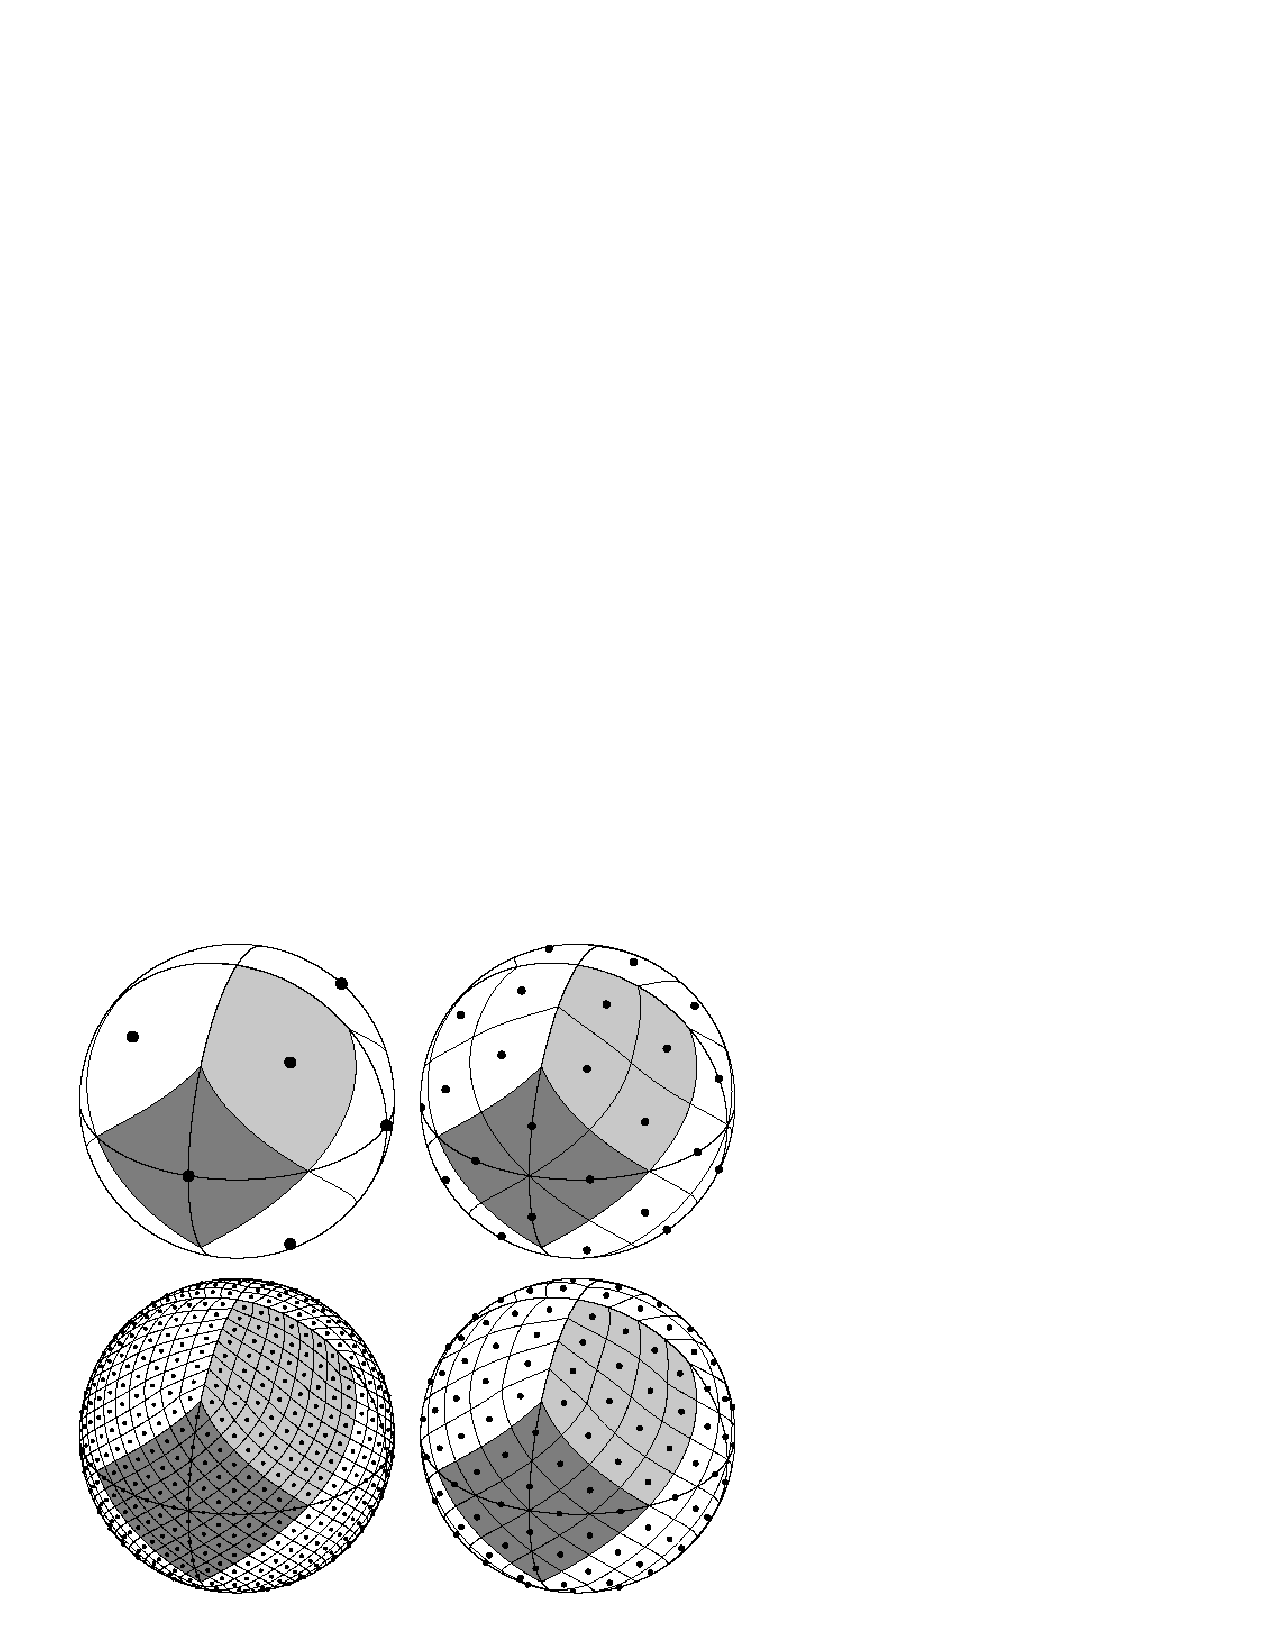
\includegraphics[width=8cm]{pixelhealpix.pdf}
\caption{The HEALPix sampling grid for four different resolutions.}
\label{pixelhealpix}
\end{figure}

The HEALPix representation (Hierarchical Equal Area isoLatitude Pixelization of a sphere) \citep{pixel:healpix}\footnote{http://healpix.jpl.nasa.gov.} 
is a curvilinear hierarchical partition of the sphere into quadrilateral pixels of exactly equal area but with varying shape. The base resolution divides 
the sphere into 12 quadrilateral faces of equal area placed on three rings around the poles and equator. Each face is subsequently divided into 
$N_{\mathrm{side}}^{2}$ pixels following a quadrilateral multiscale  tree structure (see Fig.~\ref{pixelhealpix}). The pixel centers are located 
on iso-latitude rings, and pixels from the same ring are equispaced in azimuth. This is critical for computational speed of all operations involving 
the evaluation of the spherical harmonics coefficients, including standard operations such as convolution, power spectrum estimation, and so on.  
HEALPix is a standard pixelization scheme in astronomy. 

%=================================================================================================================================

\subsection{Gauss-Legendre Sky Pixelization (GLESP)}
\index{GLESP}
\label{Glesp}
\begin{figure}
\centering
\hbox{
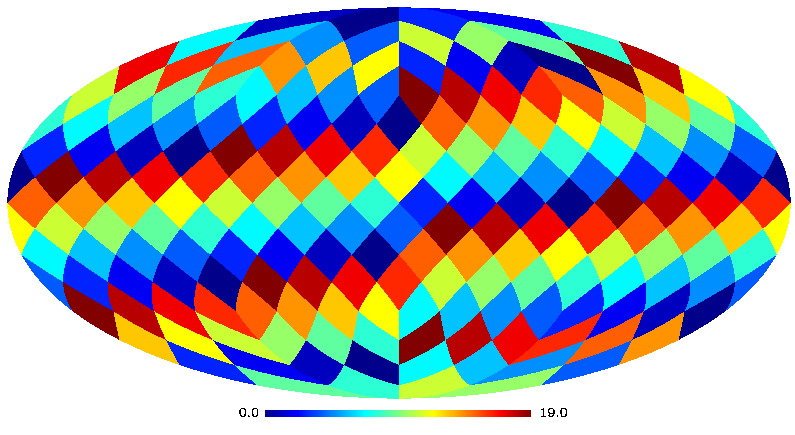
\includegraphics[width = 7.8cm]{healpix_192pix.png}
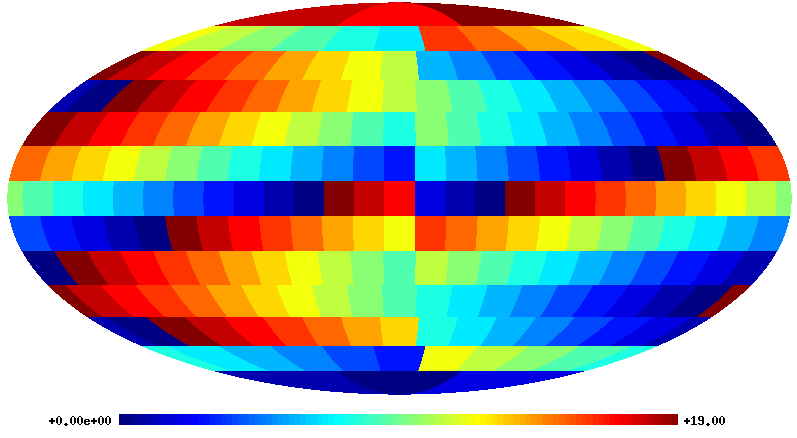
\includegraphics[width = 7.8cm]{glesp_220pix.png}
}
\caption[Comparison between Healpix and Glesp pixelization schemes.]{Comparison of pixelization schemes for a low resolution map (880 arcmin) with Healpix pixelization (on the left) and Glesp pixelization (on the right).}
\label{cmp_lowres}
\end{figure}

The principle of GLESP \citep{pixel:glesp} is to select pixels centers on points whose latitude is on the zeros of the associated Legendre's polynomial. In order to fix the longitude, 
two solutions have been built. 
The first one seeks for pixel with surfaces approximately equal. The equator is split
in $2*l+1$ pixels and other pixels bands are split in order to have pixel surfaces as closed as possible to those of the 
equatorial band. 
The second one chooses pixels with an equally spaced longitude. Pixels don't have the same surface, 
but the accuracy on spherical harmonics calculation is better.

Figure \ref{cmp_lowres} shows the shape and localization of pixels with both Healpix and GLESP scheme for a  low resolution map. 
The difference in the shape of the pixels is clearly shown. There are 16 rings and 192 pixels for the Healpix scheme, and 13 rings and 220 pixels for the GLESP one.

%=================================================================================================================================

\section{Spherical Harmonics}
\label{alm}
\index{spherical harmonics}

In the following,  the $\hat{ }$ notation will be used to denote the spherical harmonics coefficients of a function. 
Any function $f(\theta,\vartheta) \in L_2(S^2)$ on the sphere $S^2$ in $\RR^3$ can be decomposed into spherical harmonics:
\begin{eqnarray}
\label{decomp_alm}
f(\theta,\vartheta)=\sum_{l=0}^{+\infty}\sum_{m=-l}^{l} \hat{f}_{lm}Y_{lm}(\theta,\vartheta) ,
\end{eqnarray}
where  $Y_{lm}$ are the spherical harmonics defined by:
\begin{eqnarray}
\label{def_ylm}
Y_{lm}(\theta,\vartheta)=\sqrt{\frac{2l+1}{4\pi}\frac{(l- \abs{m} )!}{(l+ \abs{m} )!}} P_{lm}(\cos\vartheta)e^{im\theta},
\end{eqnarray}

$P_{lm}$ are the  associated Legendre functions (or polynomials) defined by the following differential equation:
\begin{eqnarray}
\label{def_poly_legendre}
\frac{d}{dt} \left[     (1-t^2)   \frac{d}{dt} P_{lm}  \right]   + \Big( l(l+1) - \frac{m^2}{1-t^2}\Big) P_{lm} = 0  .
\end{eqnarray}

These functions are related to the Legendre polynomials $P_{l}$ by 
\begin{eqnarray}
P_{lm}(t)  = (-1)^m (1-t^2)^{m/2}\frac{d^m}{dt^m}P_l(t) ,
\label{def_poly_leg}
\end{eqnarray}
where  $P_l$  is:
\begin{eqnarray}
P_{l}(t)  =\frac{1}{2^l l!}  \frac{d^l}{dt^l} (t^2-1)^l .
\label{def_pl}
\end{eqnarray}

Furthermore, an important property of the Legendre polynomials is that they are orthogonal:  
\begin{eqnarray}
\label{ortho_harm_sph}
\sum_{l\in\mathbb{N}} \sum_{|m|\leqslant l} Y^*_{lm}({\boldsymbol \omega}') \ Y_{lm}({\boldsymbol \omega}) = \delta({\boldsymbol \omega}' - {\boldsymbol \omega}) .
\end{eqnarray}
with ${\boldsymbol \omega} = (\theta,\vartheta)$ et ${\boldsymbol \omega}' = (\theta',\vartheta')$



\section{Multiscale methods on the sphere}
\label{intro_multi_sph}

\subsection{Wavelets on the sphere}
\index{wavelet}

Many wavelet transforms on the sphere have been proposed in the past years. Using the lifting scheme \citep{wave:sweldens95a} developed 
an orthogonal Haar wavelet transform on any surface, which can be directly applied on the sphere. Its interest is however relatively 
limited because of the poor properties of the Haar function and the problems inherent to orthogonal transforms. 
More interestingly, many papers have presented new continuous wavelet transforms \citep{wave:antoine99,wave:tenerio99,wave:cayon01,wave:holschneider96}. 
These works have been extended to directional wavelet transforms \citep{wave:antoine01,wave:hobson04}. All these continuous wavelet 
decompositions are useful for data analysis, but cannot be used for restoration purposes because of the lack of an inverse transform. 
\citep{freeden97} and \citep{freeden98} proposed the first redundant wavelet transform, based on the spherical harmonics transform, 
which presents an inverse transform. \citep{starck:sta05_2} proposed an invertible isotropic undecimated wavelet transform (UWT) 
on the sphere, also based on spherical harmonics, which has the same property as the isotropic undecimated wavelet  transform, i.e.\ the sum of the wavelet scales 
reproduces the original image. A similar wavelet construction \citep{marinucci08,fay08a,fay08} used the so-called needlet filters. 
\citep{wiaux08} also proposed an algorithm which permits to reconstruct an image from its steerable wavelet transform. Since reconstruction algorithms 
are available, these new tools can be used for many applications such as denoising, deconvolution, component separation 
\citep{starck:yassir05,bobin-gmca-cmb,delabrouille08} or inpainting \citep{inpainting:abrial06,starck:abrial08}.
\index{needlet}

The \mrs package offers an implementation of an isotropic wavelet transform on the sphere. Its properties are similar to those of the \og{}\`a trous \fg{} 
algorithm and therefore should be very useful for data denoising and deconvolution. This algorithm, described in chapter~\ref{ch_mms}, is directly derived
from the FFT-based wavelet transform proposed in \citep{starck:sta94_3} for aperture synthesis image restoration. It is relatively close to the Freeden and 
Maier \citep{freeden98} method, except that the reconstruction process is as straightforward as in the \og{}\`a trous \fg{} algorithm (i.e. the sum of the scales 
reproduces the original data). This wavelet transform can also be easily extended to a pyramidal wavelet transform, which may be very important for 
larger data sets such such as from the Planck experiment.

\subsection{Ridgelets and Curvelets on the sphere}
 \index{ridgelet}
 \index{curvelet}
In this area, further insight will come from the analysis of full-sky data mapped to the sphere thus requiring the development of a curvelet 
transform on the sphere. The \mrs package offers an implementation of ridgelet and curvelet transforms for spherical maps. Those implementations 
are derived as extensions of the digital ridgelet and curvelet transforms described in \citep{starck:sta01_3}. The implemented undecimated isotropic 
wavelet transform on the sphere and the specific geometry of the Healpix sampling grid are important components of the present implementation of 
curvelets on the sphere. \\
 
Further motivation for developing these multiscale methods on the sphere follows from the results obtained in different data processing applications. 
As described in chapter~\ref{ch_restore}, the \mrs package provides the necessary tools to experiment with these  spherical multiscale transforms in 
denoising applications, for instance using the Combined Filtering Method, which allows us to filter data on the sphere using both the Wavelet and the 
Curvelet transforms. The analysis of multichannel data mapped to the sphere, a problem encountered for instance in the processing of WMAP and Planck 
observations, is another issue that is shown to benefit from the developed multiscale representations on the sphere. This is reported in chapter~\ref{ch_mrs_ica} 
which is dedicated to describing some methods in multichannel data analysis extended to spherical maps which are implemented in the \mrs package.  




 